% !TEX root = ../main.tex
\chapter{Requirements and Design}
\label{Requirements and Design}
In this project, a model of a rural electricity network that is disconnected to the grid is expected to be modeled. To allow the network to be scalable, the network is holonic in structure and consist of communities of "smart households" which can generate and utilise electricity depending on their demand and generation profiles. Therefore the simulator was required to have the following features:
\begin{itemize}
  \item Multiple Forms of Generation: Renewable and Non-renewable generators which can operate continuously or discontinuously
  \item Realistic Generator Models: Programmable variable generation power output to simulate wind and solar power
  \item Multiple demand centres: the simulation will be of one or more communities operating with a number of households/businesses requiring electricity
  \item Self organising by the system to allocate the available power fairly to all users
  \item Presage 2: The simulation will be programmed in Java using Presage 2.
\end{itemize}

As this was a simulation implemented in Presage 2, there were no specific requirements which must be adhered to with regards to speed, portability and performance.  

The simulation was developed using Presage 2, with the hope that a network of Decentralised Community Energy Systems can be simulated, and an algorithm for fairly allocating available generation to demand will be implemented. It is assumed that no cheating will take place.

\section*{Model Design}
To allow communities to work as holonic systems, communities will be created and simulated akin to the simplified model in Figure \ref{fig:SimpleModel}. The Agents in this case are reprsented by the Circles labeled A-H, with various demand/generation equipment connected to the Agents. The Agents are connected to a Virtual Agent or a Parent Agent represented by the single black dot that all Agents on the periphery are connected to in Figure \ref{fig:SimpleModel}.

\clearpage
\begin{figure}[h!]
	\centering
	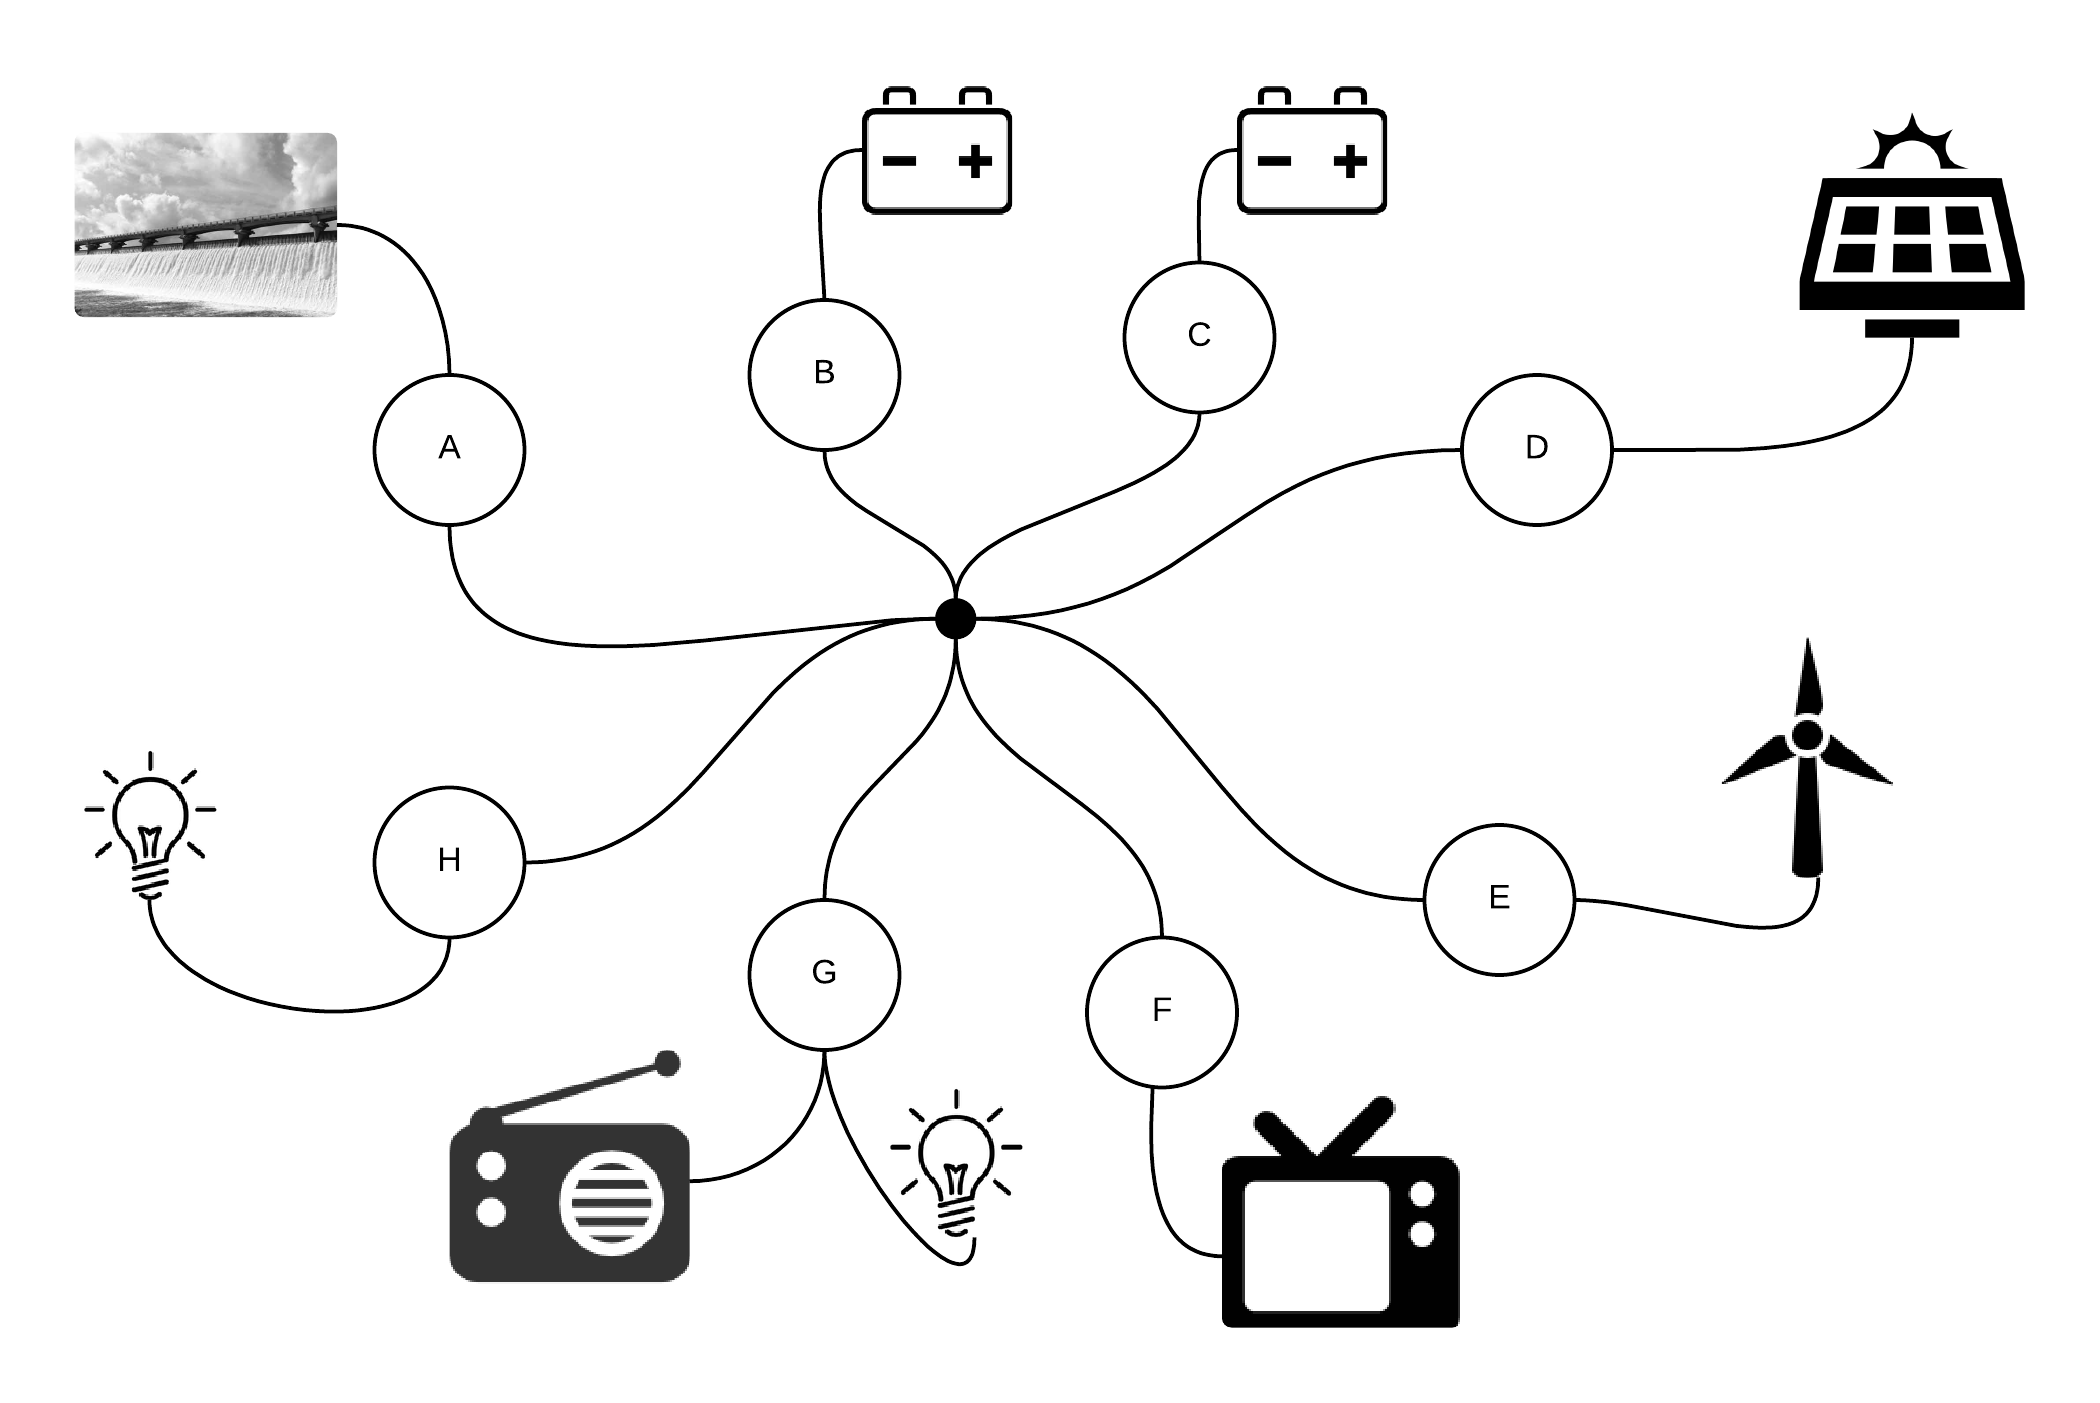
\includegraphics[scale=0.8]{Images/Model.png}
	\caption{A simplified model diagram}
	\label{fig:SimpleModel}
\end{figure}

Agents that group together are connected to a central virtual agent to allow the agents to form a community. These communities can further connected to another virtual agent to form even larger communities demonstrated in Figure \ref{fig:SimpleModel2}. 

\begin{figure}[h!]
	\centering
	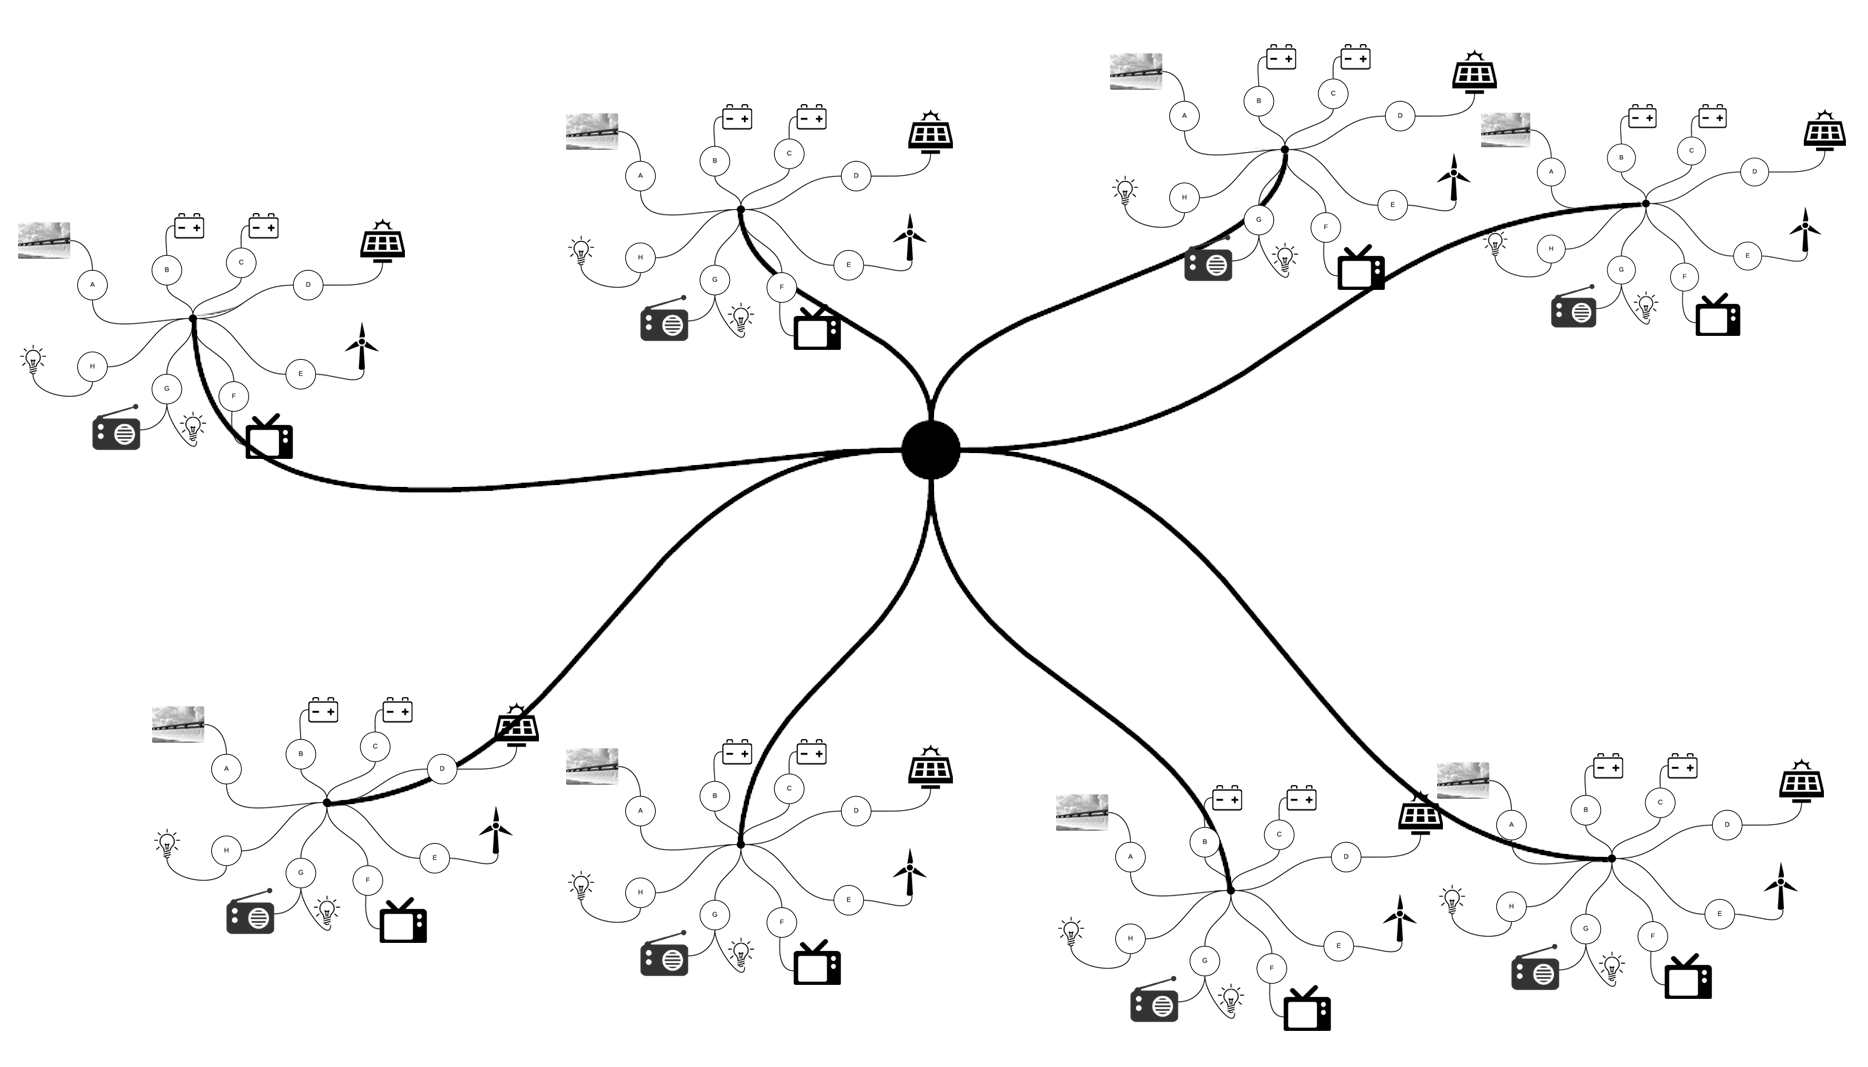
\includegraphics[scale = 0.9]{Images/Model2.png}
	\caption{A simplified network model diagram}
	\label{fig:SimpleModel2}
\end{figure}


\subsection*{Design and Model Assumptions}
To simplify the implementation of the model, a number of assumptions will be made in the design process:
\begin{itemize}
	\item No losses would be incurred by the network
	\item All load on the network will be purely resistive
	\item All generation will act as negative load
	\item Only basic appliances such as phones, lights and fridges will be connected to the vast majority of households. 
\end{itemize}

\subsection*{Types of Agents}
Presage's main components are Agents, which are the actors which can act on the environment.
\subsubsection*{Virtual Agents}
Virtual Agents represents all connected sub-communities or Agents in community of Virtual Agents. These Agents will be responsible for enforcing quotas on connected sub-communities or Agents and collecting Generation for the Common Pool. 

\subsubsection*{Prosumer Agents}
Agents represent the most "elementary" system such as generators, households, businesses and other demand centres.

\subsection*{Agent Properties}
Agent Properties represent the information that is to be relayed to the Community or Institution that the Agent is part of.
\paragraph*{Demand} - All Agents will also have the Demand property which represents aggregated electricity consumption at a point of connection. Assumed demand curves will be produced from survey data of potential customers in the area for the initial testing. Should the survey data not be available for the area, a reasonable approximation will be made based a predicted usage habits of the wider local population.

It is anticipated that the final simulation will have a desired demand profile that each agent will aim to have. 

For Virtual Agents, this property represents the aggregated Demand of all connected sub-communities or Agents and will not have any associated Demand profiles.
% However, the change in demand profile due to appropriation of energy must be able to satisfy the expected behavioral habits of the local inhabitants. These habits should include restrictions such as no trading during hours of sleep for households. What the habits will be, and how this will be implemented will be determined after some additional research into the area.

\paragraph*{Generation} - All Agents will have a Generator property which will allow all agents to generate power. For Virtual Agents, this property represents the aggregated Generation of all connected sub-communities or Agents. Four types of generator properties will be implemented in this simulation model for Prosumer Agents: 

\begin{itemize}
  \item Hydro-electric - a constant source of energy based on a mixture of historical data and projections.
  \item Solar - a source of energy following the typical output profile of a solar panel connected to households.
  \item Wind - a source of energy which will be highly variable in output.
  \item Diesel - a constant source of energy.
\end{itemize}

With the power output of renewable sources of energy such as wind and solar being non-predictable in nature, one of two approach will need to be undertaken to model these sources:
\begin{itemize}
  
  \item A probabilistic generating factor is applied to the generators. This is a constant amount of power each solar panel or wind turbine is assumed to produce during some hours of the day that is to be determined. 
  
  \begin{itemize}
    \item If this method is to be used, the model needs to be implemented in such a way to allow dynamic load-shedding and load-dumping.  
  \end{itemize}
  
  \item A probabilistic generation power output curve based on the least sunny / least windy days
  
  \begin{itemize}
    \item If this method is to be used, sufficient weather and generation data will need to be obtained to implement this method
  \end{itemize}

\end{itemize}

Both methods are in use by distribution networks in the UK for assessing network congestion \cite{IPSA-web-constraint:2015}. \

\paragraph*{Storage} - Storage devices will be batteries of various types that can be connected to the network. For the purpose of this project, it will be assumed that all Prosumer Agents will have one of these to allow allocation of electricity on a hourly basis.

The Storage property should be designed have the capability to prioritise the allocation of its stored energy for certain Agents. For example, the energy output of Storage-only agents could be made to always prioritise the households they are attached to. If the battery box is communal or belongs to a centralised entity such as an e.quinox Energy Kiosk, then no priority will be attached.

\section*{Simulation with Presage 2}
For the initial implementation and testing, the model will only contain two levels of Aggergation (see figure below): \\\\

\begin{center}
Include figure here.
\end{center}

During a round, Agents are expected to publish their Demand/Generation to their Community or Parent Agent. The Parent Agent aggregates this Demand/Generation and publishes to the Supervisor. The Supervisor aggregates the total Demand/Generation and appropriates the electricity fairly.

\section*{Fair Appropriation of the Common Pool Resource}
